\documentclass{article}
\usepackage[utf8]{inputenc}
\usepackage[margin=0.70in]{geometry}
\usepackage{hyperref}
\usepackage{graphicx}
\usepackage{authblk}
\usepackage{subfig}
\usepackage{indentfirst}
\usepackage{minted}

\title{Program Assignment 2: GPGPU-Sim}
\author{Brian Park}
\affil{North Carolina State University, Computer Engineering 786}
\date{March 2023}

\begin{document}

\maketitle

\section{Task 1: Instruction Semantic}
% task1: 25 points, 10 points for each test case(totally 2 test case), 5 points for discussion in your report
For this task, I chased down where possible the add instruction would be implemented \verb|instructions.cc|. There were two possible options: \verb|add_impl| and \verb|addp_impl|. It seems like the p version was predicate version, so I tried modifying \verb|add_impl| and it worked. It was pretty simple to modify based on the information I knew, so it's only a one line change. I only modified the FP32 instructions to do power. 

On line 1061:

\begin{minted}{C++}[H]
void add_impl(const ptx_instruction *pI, ptx_thread_info *thread) {
...
    // data.f32 = src1_data.f32 + src2_data.f32;
    data.f32 = pow(src1_data.f32, src2_data.f32);
...
}
\end{minted}

\begin{minted}{C++}[H]
diff --git a/src/cuda-sim/instructions.cc b/src/cuda-sim/instructions.cc
index 8936fa8..dfa599b 100644
--- a/src/cuda-sim/instructions.cc
+++ b/src/cuda-sim/instructions.cc
@@ -967,7 +967,7 @@ void addp_impl(const ptx_instruction *pI, ptx_thread_info *thread) {
       data.f16 = src1_data.f16 + src2_data.f16;
       break;  // assert(0); break;
     case F32_TYPE:
-      data.f32 = src1_data.f32 + src2_data.f32;
+      data.f32 = src1_data.f32 + src2_data.f32 + src2_data.f32;
       break;
     case F64_TYPE:
     case FF64_TYPE:
@@ -1058,7 +1058,7 @@ void add_impl(const ptx_instruction *pI, ptx_thread_info *thread) {
       data.f16 = src1_data.f16 + src2_data.f16;
       break;  // assert(0); break;
     case F32_TYPE:
-      data.f32 = src1_data.f32 + src2_data.f32;
+      data.f32 = pow(src1_data.f32, src2_data.f32);
       break;
     case F64_TYPE:
     case FF64_TYPE:
\end{minted}

\section{Task 2: Benchmark Performance Study}
% task2: 20 points, 15 points for the plots, 5 points for discussion
Note that the argument \verb|-gpgpu_max_insn 100000000| was added to \verb|gpgpusim.config| to limit the number of instructions. Also, for tasks 3 and 4 use \verb|SM6_TITANX| configs.
\begin{figure}[H]
    \centerline{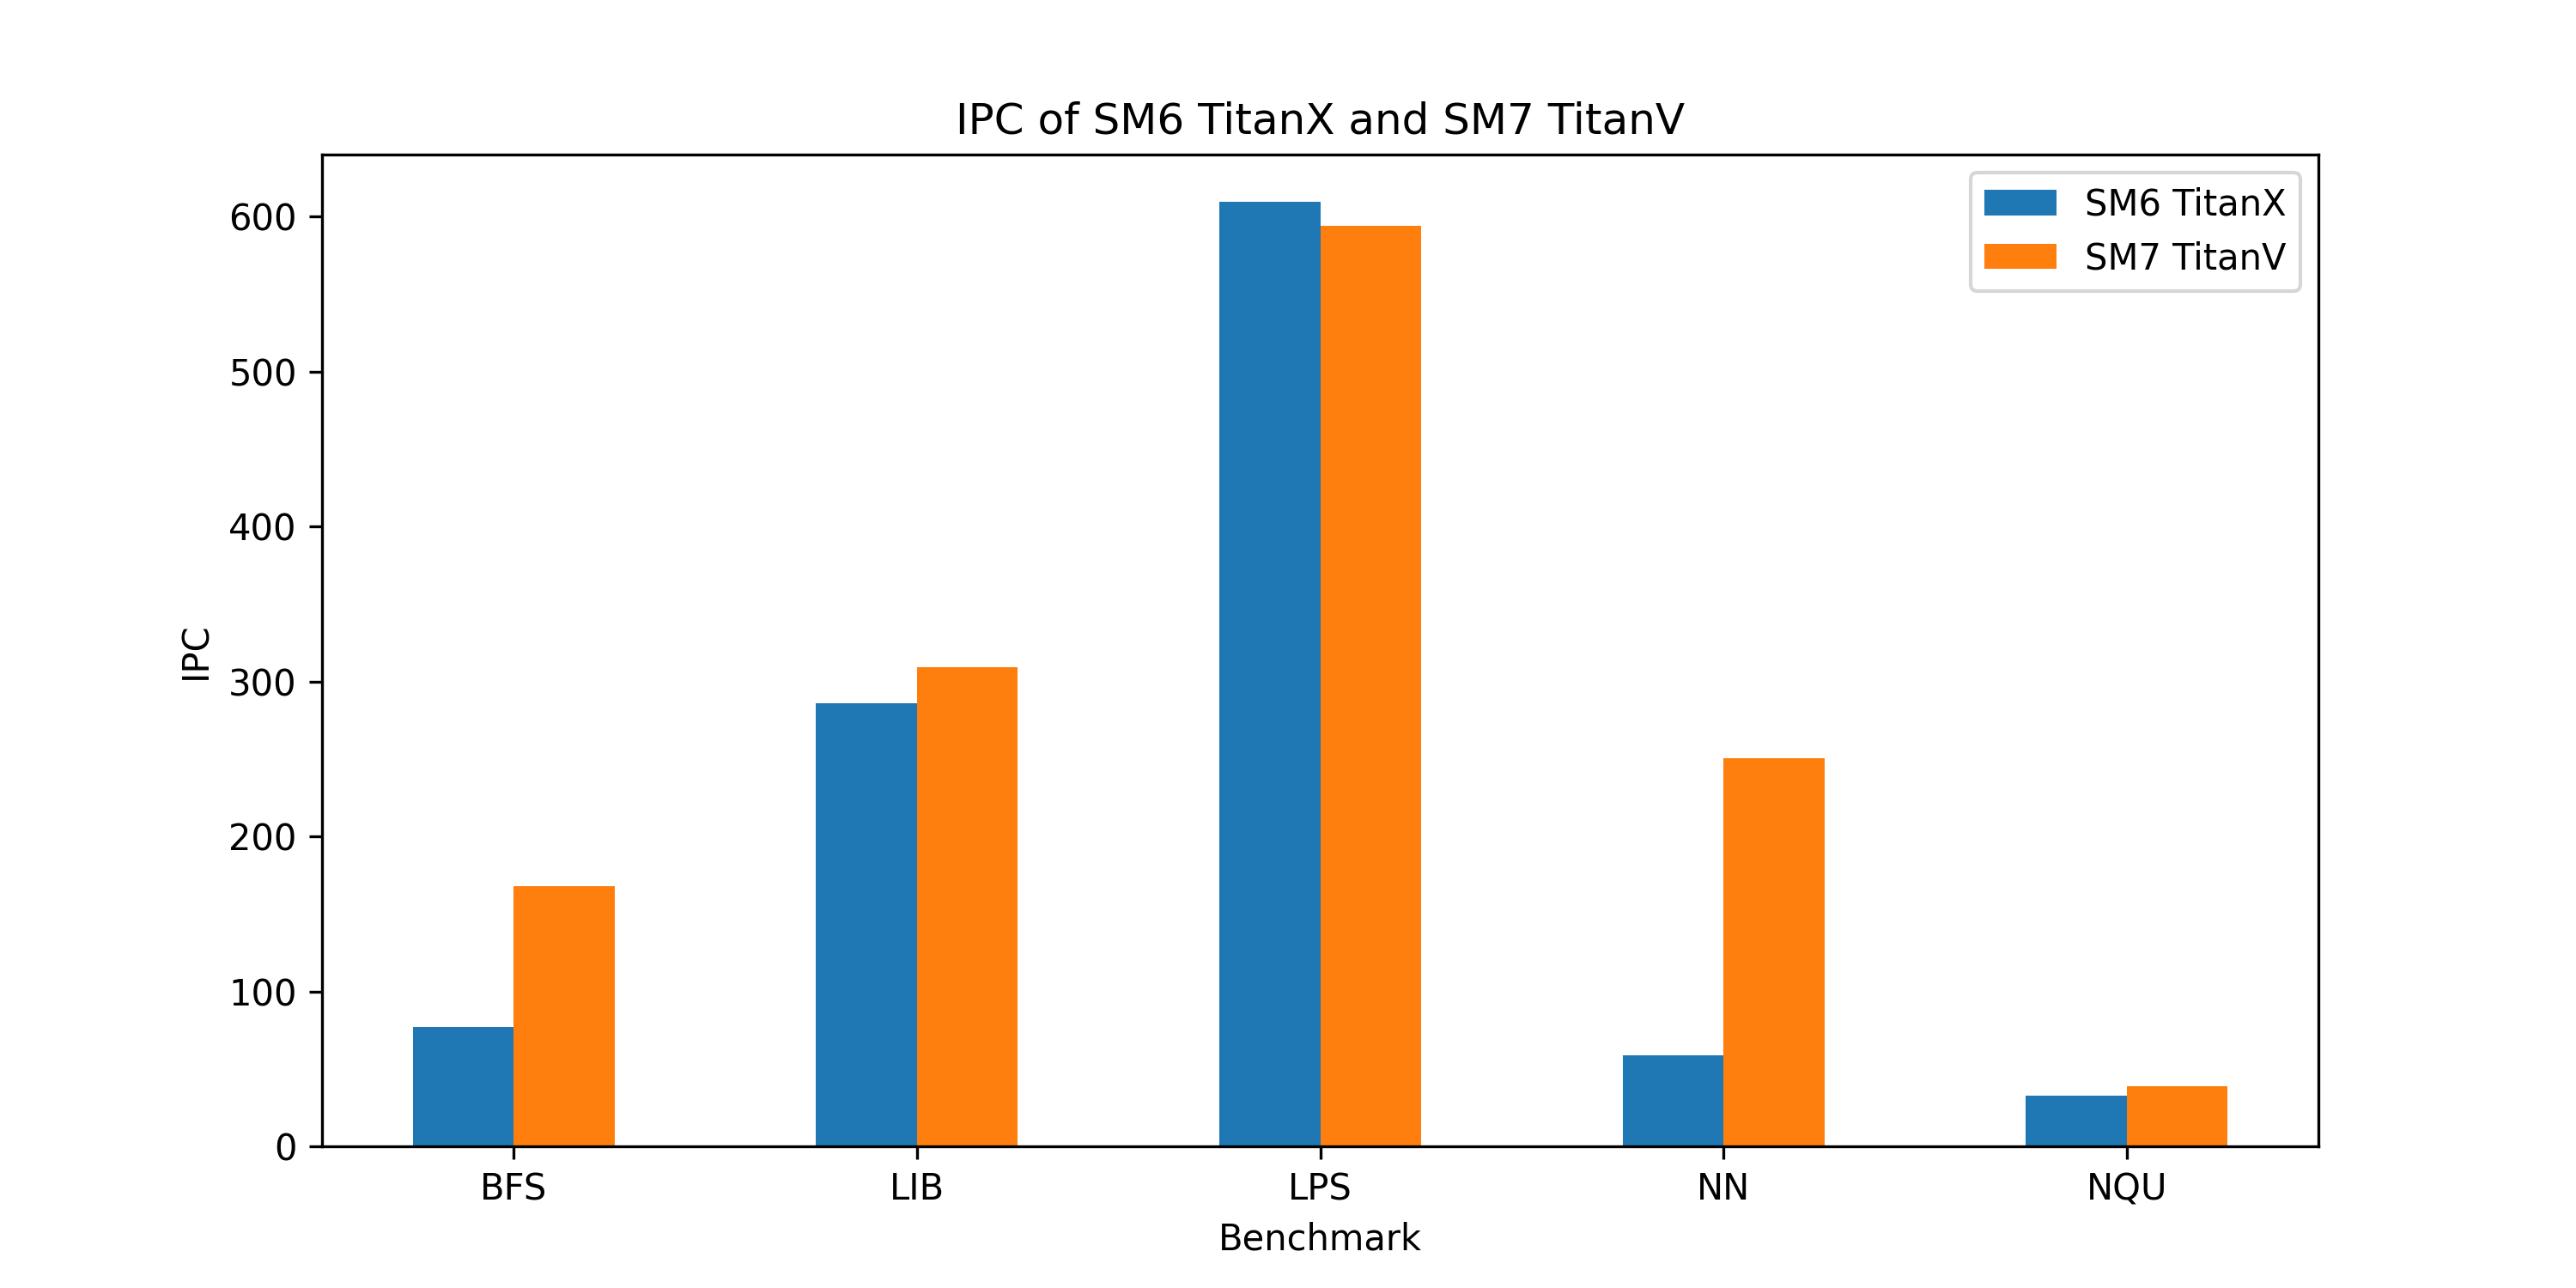
\includegraphics[width=6in]{ipc.png}}
\end{figure}

Here, we measure IPC. This indicates a higher number is better. The IPCs are abnormally high. Trusting the output of GPGPU-Sim, the only conclusion for this high IPC must be that the instructions must be decoupled per SM to give such a high IPC (instructions are aggregated across multiple SMs and divided by total number of cycles for one SM). 

Assuming that SM7 TitanV is a succeeding generation of SM6 TitanX microacrchitecture (based on the naming), we see that it outperforms SM6 TitanX on BFS, LIB, NN, and NQU. Only LPS is where SM6 is better, but only by a little bit. 

\section{Task 3: Branch Instructions and Divergence}
% task3: 30 points, 5 points for compiling your code successfully, 20 points for dumping out the counters correctly, 5 points for reporting the counters in your report.
The total number of instructions that were conditional branches turned out to be 31900 instructions, while the number of those which diverged is 19604. That means 61.45\% of the branches incurs divergence, showing that maybe this code is not optimal for GPU or needs to be carefully performance tuned in software for optimal performance. 

For sanity check, I ran this on \verb|vectorAdd.cu|, and I get only 0 conditional branches with no divergence. That sounds correct, as there are no conditional branches in vector addition and no divergence. Although there is an \verb|if (tid < n)| statement, it probably is optimized out of the compiler.

The code changed in simulator is pretty straightforward, by modifying \verb|scheduler_unit::cycle()|, I can insert conditional statements that checks the active mask whether it is set to \verb|0xffffffff| or not and whether or not the instruction to be executed is a branch instruction. Because we know warp size is 32, the active mask \verb|0xffffffff| indicates that all the threads are active and there is no divergence. Thus, if the condition is not met, then there is a diverence. The code is shown below:

\begin{minted}{C++}[H]
void scheduler_unit::cycle() {
...
  const active_mask_t &active_mask =
        m_shader->get_active_mask(warp_id, pI);      
  if (pI->op == BRANCH_OP) {}
    m_stats->conditional_branch_instr++;
    if (active_mask != 0xffffffff) {
      m_stats->conditional_branch_instr_diverged++;
    ...
    }
  }
...
}
\end{minted}

To clarify, the results can be reproduced and counters are printed as:
\begin{verbatim}
./ispass-2009-LPS > result.txt
cat result.txt | grep conditional
>>>
conditional_branch_instr  = 31900
conditional_branch_instr_diverged  = 19604
\end{verbatim}

\section{Task 4: Memory Access Space}
% task4: 25 points, 5 points for compiling your code without any errors, 15 points for dumping out the counters correctly, 5 points for reporting the counters in your report.

There are 448400 global memory accesses and 448400 local memory accesses. This aligns with what is already outputted in \verb|gpgpu_n_mem_read_global + gpgpu_n_mem_write_global| and
\\\verb|gpgpu_n_mem_read_local + gpgpu_n_mem_write_local|. Global and local memory accesses being the same shows that there is no cache reuse of the L1 or local memory.

The code modified is in \verb|ldst_unit::memory_cycle|
\begin{minted}{C++}[H]
bool ldst_unit::memory_cycle(warp_inst_t &inst,
                             mem_stage_stall_type &stall_reason,
                             mem_stage_access_type &access_type) {

  ...
    } else if (inst.space.is_global()) {  // global memory access
    // skip L1 cache if the option is enabled
    m_stats->global_memory_accesses++;
    if (m_core->get_config()->gmem_skip_L1D && (CACHE_L1 != inst.cache_op))
      bypassL1D = true;
  }

  if (bypassL1D) {
    m_stats->local_memory_accesses++;
    ...
  } 
}
\end{minted}

To clarify, the results can be reproduced and counters are printed as:
\begin{verbatim}
./ispass-2009-LPS > result.txt
cat result.txt | grep memory_accesses
global_memory_accesses  = 448400
local_memory_accesses  = 448400
\end{verbatim}

\end{document}

comp